\section{Gibbs Sampling}

  Gibbs Sampling is a special case of the Metropolis-Hastings in which the newly proposed state is accepted with probability one. With observed data $x$, say that we have calculated the $D$-dimensional posterior
  \begin{equation}
    p(\theta\,|\,x) \propto f(\theta) = p(\theta) \; p(x\,|\, \theta)
  \end{equation}

  where the parameter $\theta = (\theta^1, \ldots, \theta^D)$ is an element of the $D$-dimensional state space $\mathcal{S} = \{1, \ldots, n\}^D$ (actually, each $\theta^i$ does not need to be derived from the same $\{1, \ldots, n\}$ and we can generalize this algorithm to account for this). Remember that:
  \begin{itemize}
    \item It is hard to calculate $p(\theta\,|\,x) = p(\theta^1, \ldots, \theta^D\,|\,x)$ because calculating the constant $c$ that normalizes $f(\theta)$ is hard (since $D$ may be large). This makes it difficult to sample from the posterior.
    \item It is easy to calculate $f(\theta) = f(\theta^1, \ldots, \theta^D)$. We just don't know how to scale the individual values appropriately and so this function is useless in of itself, even though it is directly proportional to $p(\theta\,|\,x)$.
  \end{itemize}

  \begin{figure}[H]
    \centering
    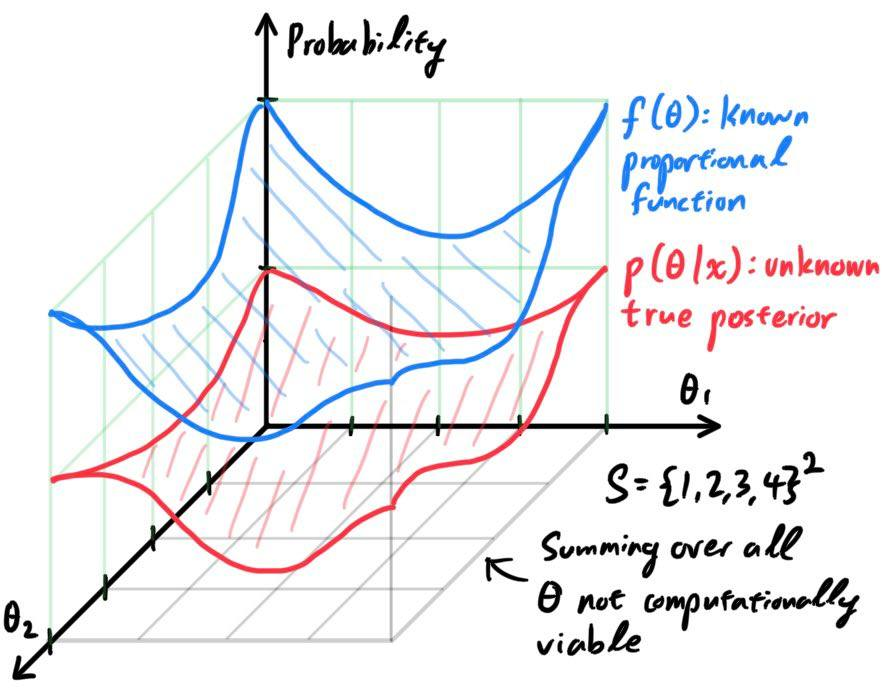
\includegraphics[width=0.7\textwidth]{img/unknown_posterior_vs_known_f.jpg}
    \caption{Comparison of unknown posterior vs known proportional function}
  \end{figure}

  With the $D$-dimensional state space $\mathcal{S}$, we construct the true transition matrix. Say that the $i$th state of the chain is located at node $\theta_i$ with given coordinates
  \begin{equation}
    \theta_i = (\theta_i^1, \theta_i^2, \ldots, \theta_i^D)
  \end{equation}

  The step to transition from this given $\theta_i$ to the next $\theta_{i+1}$ consists of two parts:
  \begin{enumerate}
    \item Pick a component index $j=d \in \{1, 2, \ldots, D\}$ uniformly at random. Many algorithms also pick $d=1$ for the first step, $d=2$ for the second, and so on.
    \begin{equation}
      p(\text{Index }d \text{ chosen}) = \frac{1}{D}
    \end{equation}
    
    \begin{figure}[H]
      \centering
      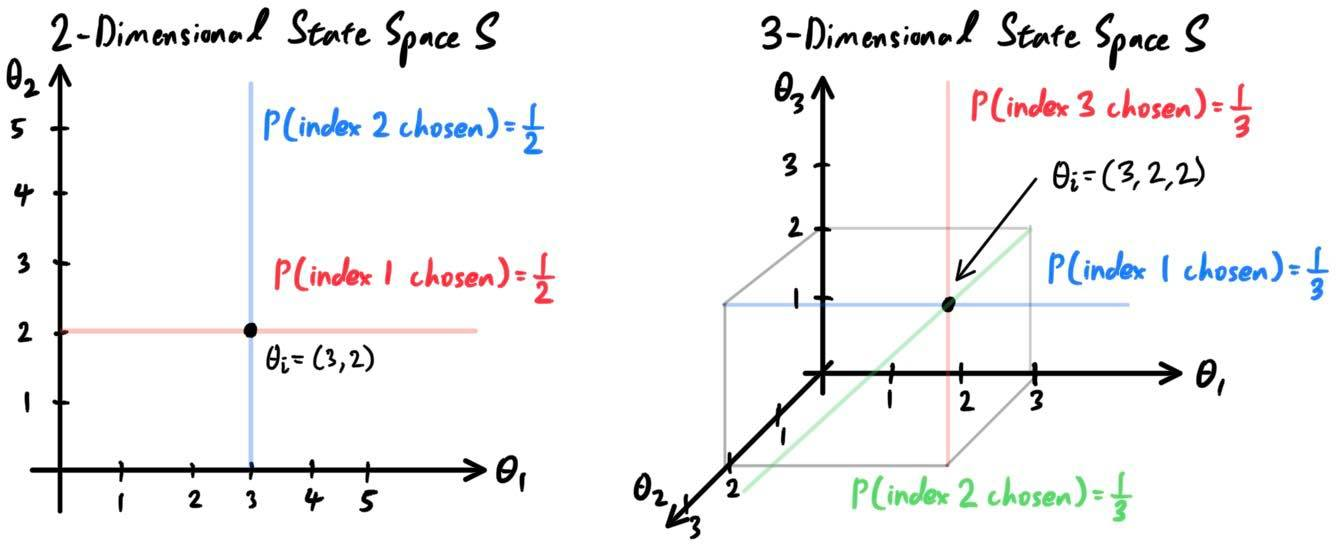
\includegraphics[width=0.8\textwidth]{img/choose_index.jpg}
      \caption{Choosing a component index in Gibbs sampling}
    \end{figure}

    \item With this well-defined $d$, we would like to update the Markov chain from state $\theta_i$ to $\theta_{i+1}$ by updating only the $d$th component of $\theta_i$, and keeping every component fixed. When $\theta_i^d$ is updated, the new $\theta_{i+1}^d$ must take some value of $k^* \in \{1, \ldots, n\}$. As expected, it chooses which value $k^*$ to update to according to the marginal distribution of $p(\theta\,|\,x)$ given $\theta_i^1, \ldots, \theta_i^{d-1}, \theta_i^{d+1}, \ldots, \theta_i^D$.
    \begin{align*}
      p(\theta_i^d \mapsto \theta_{i+1}^d = k^*\,|\, \text{Index } d \text{ chosen}) & = p(\theta_{i+1}^d = k^* \,|\,\theta_i^1, \ldots, \theta_i^{d-1}, \theta_i^{d+1}, \ldots, \theta_i^D, x) \\
      & = \frac{p(\theta_i^1, \ldots, \theta_i^{d-1}, k^*, \theta_i^{d+1}, \ldots, \theta_i^D\,|\,x)}{\sum_{k=1}^n p(\theta_i^1, \ldots, \theta_i^{d-1}, k, \theta_i^{d+1}, \ldots, \theta_i^D\,|\,x)} \\
      & = \frac{f(\theta_i^1, \ldots, \theta_i^{d-1}, k^*, \theta_i^{d+1}, \ldots, \theta_i^D)}{\sum_{k=1}^n f(\theta_i^1, \ldots, \theta_i^{d-1}, k, \theta_i^{d+1}, \ldots, \theta_i^D)}
    \end{align*}

    where the last step is justified by the proportionality of $f$ and $p$. It turns out that the probability of where $\theta_{i+1}^d$ will land on does not actually depend on where $\theta_{i}^d$ is currently.
  \end{enumerate}

  \begin{figure}[H]
    \centering
    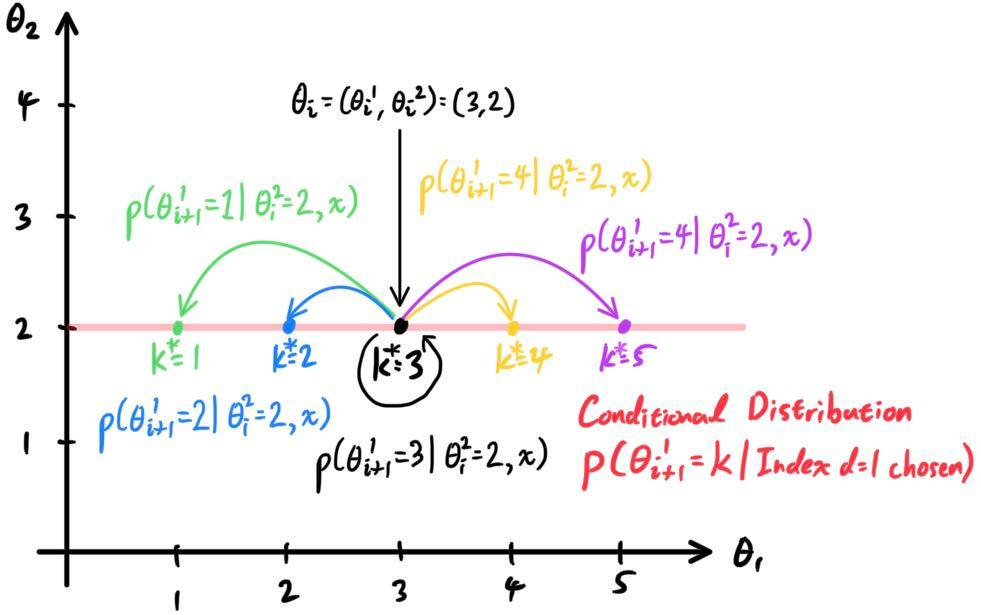
\includegraphics[width=0.7\textwidth]{img/example_gibbs_1.jpg}
    \caption{Example for $D=2, n=5$ showing possible states (within red line) that $\theta_{i+1}$ can transition to}
  \end{figure}

  Do not be daunted by the notation. Just remember that $p(\theta_{i+1}^d = k^* \,|\,\theta_i^1, \ldots, \theta_i^{d-1}, \theta_i^{d+1}, \ldots, \theta_i^D, x)$ is just the conditional probability of $p(\theta\,|\,x)$ given that every $\theta_i^j, j \neq d$ are constant. This is easily visualized by taking the 1-dimensional cross section of the density $p(\theta\,|\,x)$ defined on $\mathcal{S}$.

  \begin{figure}[H]
    \centering
    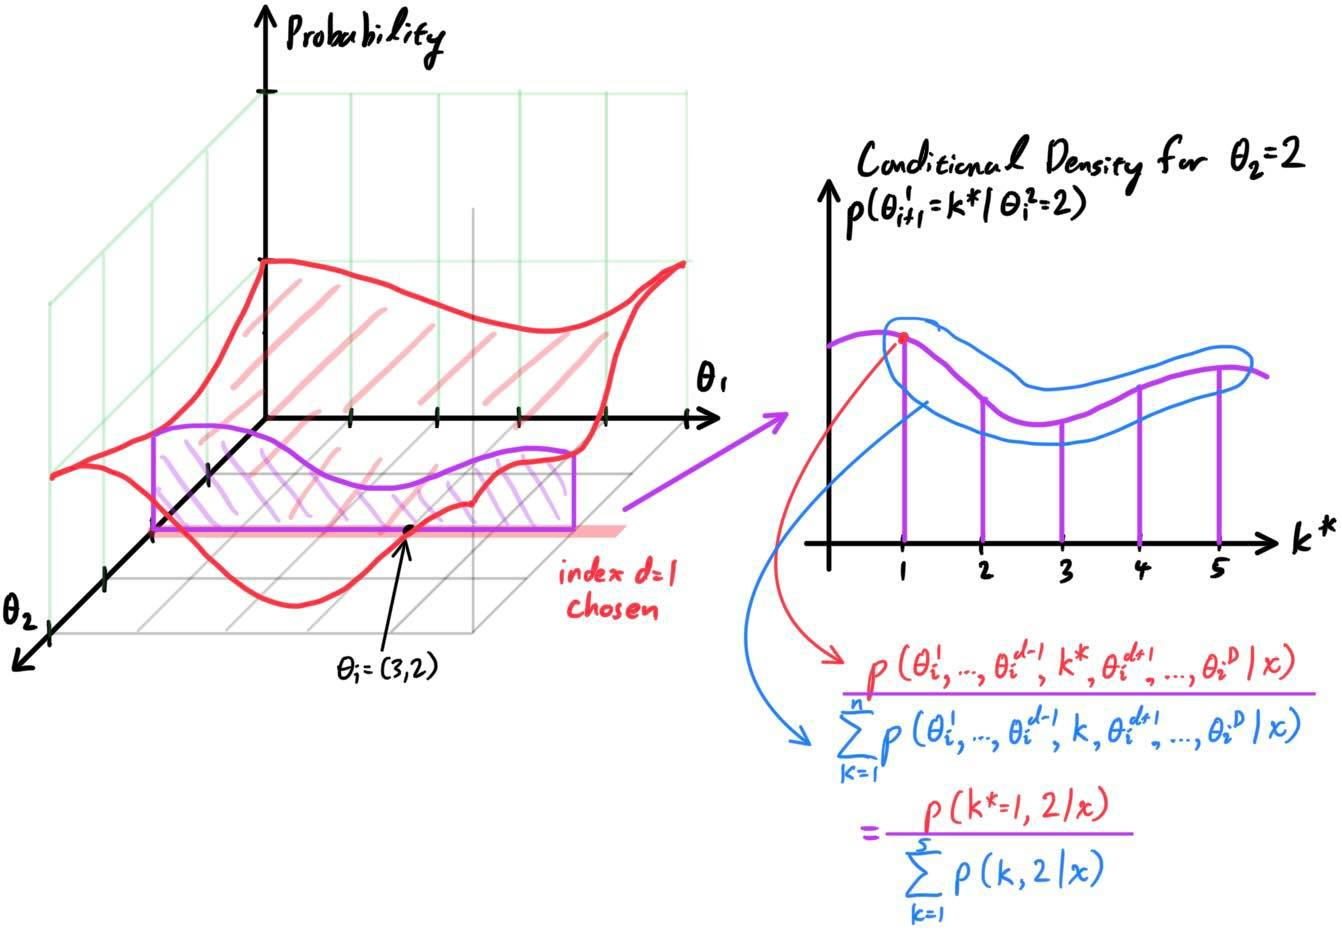
\includegraphics[width=0.8\textwidth]{img/Gibbs_step_2.jpg}
    \caption{Cross-sectional view of density in Gibbs sampling}
  \end{figure}

  Therefore, we can construct a Markov chain with the following transition probabilities. Given two states $\theta_r, \theta_s \in \mathcal{S}$, if $\theta_s$ differs in $\theta_r$ in at most one component, call it the $d$th component (i.e. $\theta_r^j = \theta_s^j$ for all $j \neq d$), then the probability of transition from $\theta_r$ to $\theta_s$ is
  \begin{align*}
    p(\theta_r, \theta_s) & = p(\theta_r^d \mapsto \theta_{s}^d\,|\, \text{Index } d \text{ chosen})\; p (\text{Index } d \text{ chosen}) \\
    & = \frac{f(\theta_r^1, \ldots, \theta_r^{d-1}, \theta_s^d, \theta_r^{d+1}, \ldots, \theta_r^D)}{\sum_{k=1}^n f(\theta_r^1, \ldots, \theta_r^{d-1}, k, \theta_r^{d+1}, \ldots, \theta_r^D)} \cdot \frac{1}{D}
  \end{align*}

  Therefore, given that the chain is in state $\theta_i = (3, 2)$ in state space $\mathcal{S} = \{1, 2, 3, 4, 5\}^2$, it may be able to get to the point in red or blue, depending on which index $d$ was chosen. But it is impossible to go to any of the yellow states, so the transition probabilities are all $0$.

  \begin{figure}[H]
    \centering
    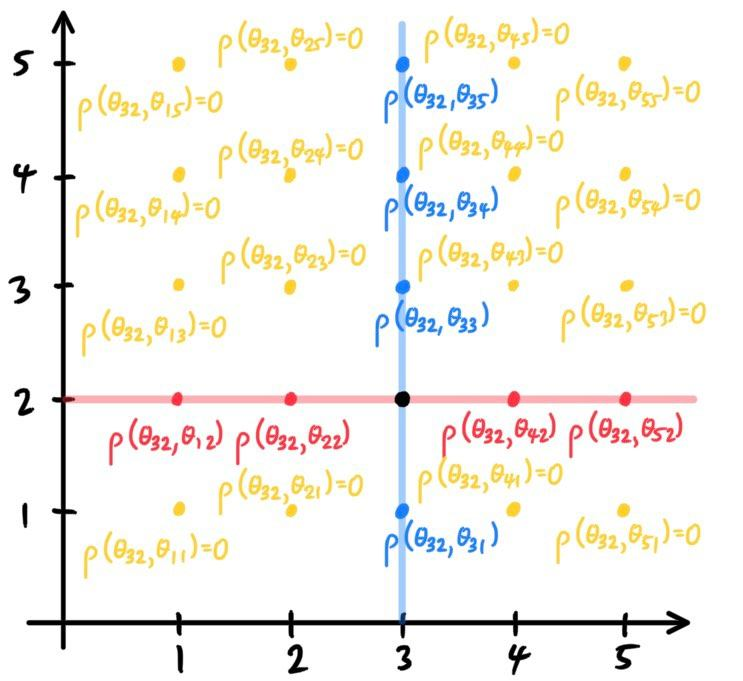
\includegraphics[width=0.6\textwidth]{img/prob_0.jpg}
    \caption{Possible transitions from state $(3,2)$ in Gibbs sampling}
  \end{figure}

  With this, we can calculate the stationary distribution by either:
  \begin{itemize}
    \item Calculating the left-eigenvector of the transition matrix defined $p(\theta_r, \theta_s)$ with eigenvalue $1$.
    \item Randomly initialize $\theta_0 = (\theta_0^1, \ldots, \theta_0^D)$ and run the chain for sufficiently long time to find out the proportion of steps in which a Markov chain lands on each $\theta \in \mathcal{S}$.
  \end{itemize}

  Now, it is easy to see why Gibbs sampling is a special case of Metropolis-Hastings. The Gibbs transition algorithm that we just mentioned is clearly a Markov chain, and within the context of Metropolis, we can interpret it as the proposal transition matrix with acceptance probability 1. By the same justification for Metropolis, we can prove that the stationary distribution of Gibbs sampling is $p(\theta\,|\,x)$.

